%------------------------------------
% To be edited
%------------------------------------
\newcommand{\documentname}{Floating point CORDIC de doble precisi\'on}
\newcommand{\crev}{0.5}
\newcommand{\documentversion}{Rev. \crev}
\newcommand{\cryear}{2016}
\hyphenation{soft-ware hard-ware}
%------------------------------------

\documentclass[10pt,a4paper]{book}
\setlength{\parindent}{0pt}
\setlength{\parskip}{1ex plus 0.5ex minus 0.2ex}
\addtolength{\headsep}{0.5cm}
\usepackage[a4paper]{geometry} %,left=2.5cm,right=3.5cm
\usepackage[colorlinks=false]{hyperref}
\usepackage[english, activeacute]{babel}
\usepackage[utf8]{inputenc}
\usepackage{graphics}
\usepackage[final]{graphicx}
\usepackage{caption}
\usepackage{subcaption}
\usepackage{float}                        %  alows using subfloat for graphics
\usepackage[maxfloats=256]{morefloats}    %  max number of floating figures ( in the appendices you have like 200)
\usepackage{rotating}
\usepackage{color}
\usepackage{longtable}
\usepackage{latexsym}
\usepackage{multicol}
\usepackage{multirow}
\usepackage{fancyhdr}
\usepackage{gensymb}                      % for degree symbol
\usepackage{listings}                     % to show source code
\lstloadlanguages{VHDL}
\usepackage{tikz}                         % for DIA graphics
\usepackage{makeidx}                      % to make the index
%%%%%%%%%\usepackage{bytefield}

% Paquetes matematicos
\usepackage{amsfonts}
\usepackage{amsmath}
\usepackage{amssymb}
\usepackage{amsthm}
\usepackage{mathrsfs}
\DeclareMathOperator\arctanh{arctanh}

\pagestyle{fancy}

%\usepackage{anysize}
%\marginsize{3cm}{4cm}{2.5cm}{3.5cm}

%---- Encabezado y pie de pagina general
\fancypagestyle{general}
{
   \fancyhf{}
   \fancyfoot{}
   \fancyhead{}
   \fancyhead[LO]{\footnotesize{\leftmark}}
   \fancyhead[RE]{\footnotesize{\rightmark}}
   \fancyhead[RO]{\footnotesize{\thepage}}
   \fancyhead[LE]{\footnotesize{\thepage}}
   \renewcommand{\headrulewidth}{0pt}
   \renewcommand{\footrulewidth}{0pt}
   }

\fancypagestyle{plain}
{
   \fancyhf{}
   \fancyfoot{}
   \fancyhead{}
   \fancyfoot[RO]{\footnotesize{\thepage}}
   \fancyfoot[LE]{\footnotesize{\thepage}}
   \renewcommand{\headrulewidth}{0pt}
   \renewcommand{\footrulewidth}{0pt}
   }

%---- Encabezado y pie de pagina de la caratula
\fancypagestyle{carat} {
   \fancyhf{}
   \fancyfoot{}
   \fancyhead{}
   \fancyhead[LO]{\scalebox{0.15}{
\includegraphics[angle=0]{./figures/logo_lab_ue_3.png}}}
   \fancyhead[RE]{}
   \fancyhead[RO]{\scalebox{0.5}{
\includegraphics[angle=0]{./figures/logo_fiuba.jpg}}}
   \fancyhead[LE]{}
   \fancyhead[CE]{}
   \fancyfoot[CO]{\textcircled{c} Lab-$\mu$E, FIUBA. \cryear.}
   \renewcommand{\headrulewidth}{0pt}
   \renewcommand{\footrulewidth}{1pt}
}

%---- Quito los encabezados y pies de pagina en las hojas vacias
\makeatletter
  \def\cleardoublepage{\clearpage\if@twoside \ifodd\c@page\else
  \vspace*{\fill}
    \thispagestyle{empty}
    \newpage
    \if@twocolumn\hbox{}\newpage\fi\fi\fi}
\makeatother

%---- Espaciado en el indice entre el numero y el titulo
\makeatletter
\renewcommand*{\l@subsection}{\@dottedtocline{1}{3.8em}{3.5em}}
\renewcommand*{\l@figure}{\@dottedtocline{1}{1.5em}{3.3em}}
\renewcommand*{\l@table}{\@dottedtocline{1}{1.5em}{2.8em}}
\makeatother

%---- Formateo del codigo VHDL
\lstset
{
   %extendedchars=true,%
   %labelstep=0,
   %labelsep=3ex,
   %frame=trbl,
   %frameround=tttt,
   %framespread=-3ex,
   %framerulecolor=colorFondoListado,
   %backgroundcolor=colorFondoListado,
   captionpos=b,
   breaklines=true,
   %linewidth=0.98\linewidth,
   %indent=5ex,
   tabsize=4,
   %labelstyle=\small\ttfamily,
   basicstyle=\scriptsize\sffamily,
   %numberstyle=\small\sffamily,
   identifierstyle=\scriptsize\sffamily,
   commentstyle=\scriptsize\itshape,
   stringstyle=\scriptsize\sffamily,
   keywordstyle=\scriptsize\bfseries\sffamily,
   ndkeywordstyle=\scriptsize\bfseries\sffamily,
   showstringspaces=false,
   flexiblecolumns=false
   visiblespaces=false
   %stringspaces=false
}

%---- Encabezado y pie de pagina por defecto
\pagestyle{general}

%---- Matematica
\newtheorem{defi}{Definici\'on}
\newtheorem{teor}{Teorema}
\newtheorem{prop}{Proposici\'on}
\newtheorem{lema}{Lema}
\newtheorem{cor}{Corolario}
\DeclareMathOperator{\sen}{sen}
\DeclareMathOperator{\supr}{sup}
\DeclareMathOperator{\sgn}{sgn}
\DeclareMathOperator{\lip}{lip}
\DeclareMathOperator{\codim}{codim}
\DeclareMathOperator{\gen}{gen}
\DeclareMathOperator{\im}{Im}
\DeclareMathOperator{\nuc}{Nu}
\DeclareMathOperator{\ind}{ind}
\DeclareMathOperator{\dom}{Dom}
\DeclareMathOperator{\real}{Real}
\DeclareMathOperator{\imag}{Imag}

%---- Para no separar en SILABAS se activa el comando siguiente
\hyphenpenalty=10000


\begin{document}

%------------------------------------------------
% 1.Introducción
%------------------------------------------------
\chapter{CORDIC}

% 1.1 Algoritmo CORDIC
\section{Algoritmo CORDIC}

El algoritmo CORDIC propuesto por Volder realizaba rotaciones en coordenadas circulares.
Partiendo de esa base es facil extender su funcionamiento para que realice rotaciones en coordenadas hiperbólicas y lineales. Para lograrlo se agrega una variables que modifica las ecuaciones y además se eligen diferentes angulos para el acumulador de angule (variable z del algoritmo).
Las ecuaciones del CORDIC completo son:
\begin{equation} \label{eq:cordic_eq}
   \begin{subequations}
      \begin{aligned}
         x_{n+1} &=  x_n - m \cdot d_n \cdot 2^{-s_{m,n}}   \\
         y_{n+1} &=  y_n + d_n \cdot 2^{-s_{m,n}}             \\
         z_{n+1} &=  z_n - d_n \cdot \alpha_{m,n}
      \end{aligned}
   \end{subequations}
\end{equation}

Donde $N$ representa la cantidad de pasos del algoritmo y se cumple que $n= 0, 1, 2, ... , N-1$. $s_{m,n}$ es una sequencia de números enteros no decreciente llamada \textit{shift sequence} y $\alpha_{m,n}$ representa los angulos rotados para las diferentes coordenadas. $d_n$ es una variable de control que maneja los sumadores/restadores.
\begin{equation} \label{eq:rotation_angle}
   \alpha_{m,n} = \dfrac {1}{\sqrt{m}} \cdot \tan^{-1}(\sqrt{m} \cdot 2^{-s_{m,n}} )
\end{equation}

Eligiendo correctamente $d_n$ y $s_{m,n}$ el algoritmo converge (ver tabla ~\ref{tab:table_shift_seq}). La tabla ~\ref{tab:table_cordic_outputs} muestra las diferentes salidas del algoritmo. En la table ~\ref{tab:table_cordic_outputs_special_cases} podemos ver las salidas del algoritmo para valores de entrada particulares, estos valores son de especial interés ya que representan operaciones matematicas difíciles de calcular.

\begin{table}[h!]
\centering
\begin{tabular}{llll}
   \hline
   Sistema de coordenadas  &  Shift sequence       &  Convergencia   &  Factor de escala                 \\ \hline \hline
   $m$                     &  $s_{m,n}$            &  $|A_0|$        &  $K_{m} (n \rightarrow \inf)$     \\ \hline
   1                       &  0,1,2, ... , n       &  $ 1.74$        &  $1.64676$                        \\ \hline
   0                       &  1,2,3, ... , n+1     &  $ 1.0 $        &  $1.0    $                        \\ \hline
   -1                      &  1,2,3,4,4, ...       &  $ 1.13$        &  $0.82816$                        \\ \hline \hline
\end{tabular}
\caption{CORDIC shift sequences}
\label{tab:table_shift_seq}
\end{table}

\begin{table}[h!]
\centering
\begin{tabular}{clll}
   \hline
   $m$   &  Modo     &  Entradas          & Salidas                                                \\ \hline \hline
   1     &  rotation &  $x_0 = x$         & $x_N = K_1 \cdot (x \cos\theta - y \sin\theta)$        \\
         &           &  $y_0 = y$         & $y_N = K_1 \cdot (y \cos\theta + x \sin\theta)$        \\
         &           &  $z_0 = \theta$    & $z_N = 0$                                              \\ \hline
   1     &  vectoring&  $x_0 = x$         & $x_N = K_1 \cdot sign(x) \cdot \sqrt{x^2+y^2}$         \\
         &           &  $y_0 = y$         & $y_N = 0$                                              \\
         &           &  $z_0 = \theta$    & $z_N = \theta + \tan^{-1}(y/x)$                        \\ \hline
   0     &  rotation &  $x_0 = x$         & $x_N = x $                                             \\
         &           &  $y_0 = y$         & $y_N = y + x \cdot z$                                  \\
         &           &  $z_0 = \theta$    & $z_N = 0$                                              \\ \hline
   0     &  vectoring&  $x_0 = x$         & $x_N = x$                                              \\
         &           &  $y_0 = y$         & $y_N = 0$                                              \\
         &           &  $z_0 = z$         & $z_N = z + y / x$                                      \\ \hline
   -1    &  rotation &  $x_0 = x$         & $x_N = K_{-1} \cdot (x \cosh\theta + y \sinh\theta)$   \\
         &           &  $y_0 = y$         & $y_N = K_{-1} \cdot (y \cosh\theta + x \sinh\theta)$   \\
         &           &  $z_0 = \theta$    & $z_N = 0$                                              \\ \hline
   -1    &  vectoring&  $x_0 = x$         & $x_N = K_{-1} \cdot sign(x) \cdot \sqrt{x^2-y^2}$      \\
         &           &  $y_0 = y$         & $y_N = 0$                                              \\
         &           &  $z_0 = \theta$    & $z_N = \theta + \tanh^{-1}(y/x)$                       \\ \hline
\end{tabular}
\caption{Salidas del algoritmo CORDIC.}
\label{tab:table_cordic_outputs}
\end{table}


\chapter{Algoritmo de Briggs para ln(x)}

Si se encuentra una secuencia $d_k$ tal que la productoria de $x$ con $(1+d_k 2^{-k})$ es cercana a 1 entonces vale que:

\begin{equation} \label{eq:briggs_ln}
   \begin{subequations}
      \begin{aligned}
         x \prod_{k=1}^{n} (1+d_k 2^{-k}) \approx 1     \\
         ln(x) \approx - \sum_{k=1}^{n} \ln(1+d_k 2^{-k})
      \end{aligned}
   \end{subequations}
\end{equation}


\chapter{BKM}

   \section{Origenes}

   Consideremos el paso básico del algoritmo CORDIC en modo trigonométrico (con m=1).
   Si definimos el número complejo $E_n = x_n + j \, y_n$ con $j=\sqrt{-1}$, obtenemos $E_{n+1} = E_n (1+j \, d_n 2^{-n})$, esta relación es similar al paso básico del algorithmo de Briggs.
   Esta similitud nos lleva a una generalización de ese algoritmo: podriamos realizar multiplicaciones por terminos $(1+d_n 2^{-n})$, donde los $d_n$s son números complejos elejidos de tal manera que la multiplicación por $d_n$ pueda reducirce a unas pocas sumas.
   Entonces se define el algoritmo BKM de la siguiente manera:

\begin{equation} \label{eq:bkm_eqs}
   \left\{
      \begin{aligned}
         E_{n+1} &= E_n \cdot (1 + d_n 2^{-n})   \\
         L_{n+1} &= L_n - \ln(1 + d_n 2^{-n})
      \end{aligned}
   \right.
\end{equation}

   con $d_n \in \{ 0, \pm 1, \pm j, \pm 1 \pm j\}$ y $\ln z$ es el número complejo $t$ tal que $\exp{t} = z$ y cuya parte imaginaria está entre $-\pi$ y $\pi$.


\section{E-mode}

   Encontrar una sequencia de $d_n$ tal que $L_n \rightarrow 0$ entonces $E_n \rightarrow E_1 e^{L_1}$.

\begin{equation} \label{eq:bkm_E_mode}
   \left\{
      \begin{aligned}
         E_n & \rightarrow E_1 e^{L_1} \\
         L_n & \rightarrow 0
      \end{aligned}
   \right.
\end{equation}

   \subsection{Canal de datos}
\begin{equation} \label{eq:bkm_eqs_E}
   \left\{
      \begin{aligned}
         E_{n+1}^x &= E_n^x + ( d_n^x E n^x - d_n^y E_n^y ) \,2^{-n} \\
         E_{n+1}^y &= E_n^y + ( d_n^x E n^y + d_n^y E_n^x ) \,2^{-n}
      \end{aligned}
   \right.
\end{equation}

   \subsection{Canal de control}
\begin{equation} \label{eq:bkm_eqs_l}
   \left\{
      \begin{aligned}
         l_n         &= 2^n L_n                                                                             \\
         l_{n+1}     &= 2 l_n   - 2^{n+1} \ln( 1 + d_n 2^{-n} )                                             \\
         l_{n+1}^x   &= 2 l_n^x - 2^{n}   \ln[ 1 + d_n^x \, 2^{-n+1} - ({d_n^x}^2 + {d_n^y}^2) \, 2^{-2n} ] \\
         l_{n+1}^y   &= 2 l_n^y - 2^{n+1} d_n^y \, \arctan{ \left( \frac{2^{-n}}{1+d_n^x 2^{-n}} \right) }
      \end{aligned}
   \right.
\end{equation}

\begin{equation} \label{eq:bkm_eqs_l_limit}
   2^{n} \ln( 1 + d_n 2^{-n} ) \rightarrow 1 \qquad as \,\, n \rightarrow +\infty
\end{equation}



\section{L-mode}
   Encontrar una sequencia de $d_n$ tal que $E_n \rightarrow 1$ entonces $L_n \rightarrow L_1 + \ln(E_1)$.

\begin{equation} \label{eq:bkm_E_mode}
   \left\{
      \begin{aligned}
         E_n & \rightarrow 1 \\
         L_n & \rightarrow L_1 + \ln(E_1)
      \end{aligned}
   \right.
\end{equation}

   \subsection{Canal de datos}
\begin{equation} \label{eq:bkm_eqs_L}
   \left\{
      \begin{aligned}
         L_{n+1}^x &= L_n^x - \frac{1}{2} \ln[ 1 + d_n^x \, 2^{-n+1} - ({d_n^x}^2 + {d_n^y}^2) \, 2^{-2n} ] \\
         L_{n+1}^y &= L_n^y - d_n^y \, \arctan{ \left( \frac{2^{-n}}{1+d_n^x 2^{-n}} \right) }
      \end{aligned}
   \right.
\end{equation}

   \subsection{Canal de control}
\begin{equation} \label{eq:bkm_eqs_e}
   \left\{
      \begin{aligned}
         e_n         &= 2^n (E_n - 1)                                            \\
         e_{n+1}     &= 2 (e_n   + d_n) + d_n e_n 2^{-n+1}                       \\
         e_{n+1}^x   &= 2 (e_n^x + d_n^x) + (d_n^x e_n^x - d_n^y e_n^y) 2^{-n+1} \\
         e_{n+1}^y   &= 2 (e_n^y + d_n^y) + (d_n^y e_n^x + d_n^x e_n^y) 2^{-n+1} \\
      \end{aligned}
   \right.
\end{equation}

\chapter{Architecture}

   \section{BKM Float}

   \section{BKM Fixed}

      \begin{figure}[h]
         \centering
         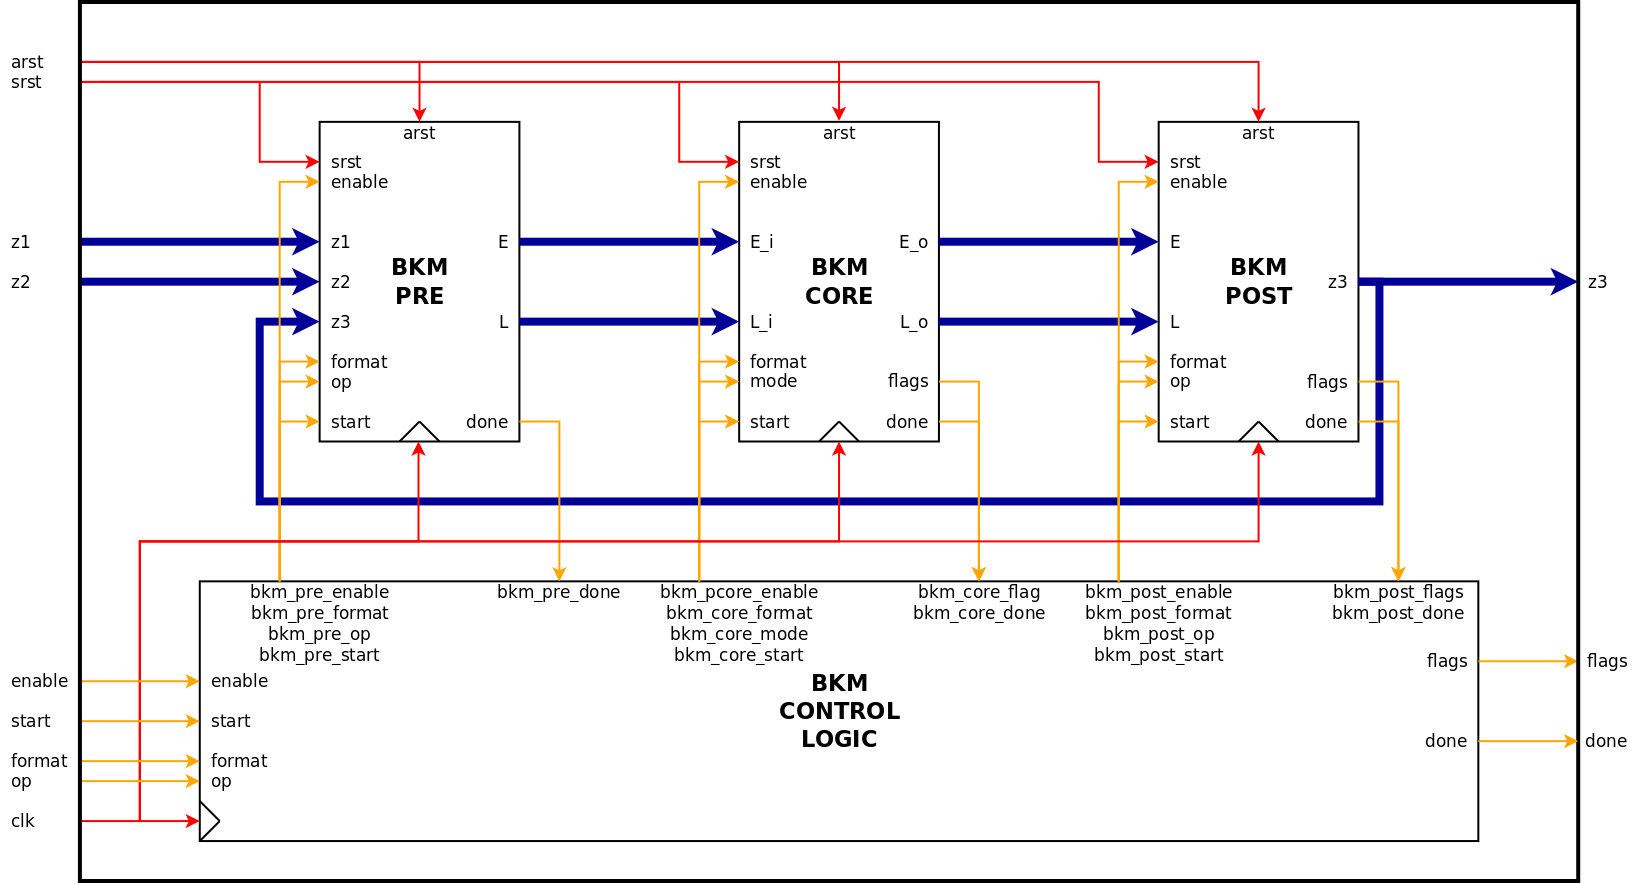
\includegraphics[width=1.0\textwidth]{./figures/bkm_fixed.png}
         \caption{Arquitecture del bloque BKM fixed.}
         \label{fig:bkm_fixed}
      \end{figure}

      \begin{table}[h]
      \centering
      \begin{tabular}{lccl}
         \hline
         Puerto            &  Tama\~no    &  Direcci\'on    &  Descripci\'on                                                  \\ \hline \hline
         \verb|clk      |  &  1  bit      &  Input          &  Clock signal                                                   \\ \hline
         \verb|arst     |  &  1  bit      &  Input          &  Active high asynchronous reset signal                          \\ \hline
         \verb|srst     |  &  1  bit      &  Input          &  Active high synchronous reset signal                           \\ \hline
         \verb|enable   |  &  1  bit      &  Input          &  Active high enable signal                                      \\ \hline
         \verb|start    |  &  1  bit      &  Input          &  Active high start signal                                       \\ \hline
         \verb|format   |  &  2  bit      &  Input          &  Format specifier (0/1): MSB for complex/real, LSB for 64/32 bits\\ \hline
         \verb|op       |  &  5  bits     &  Input          &  Operation code                                                 \\ \hline
         \verb|x_1      |  &  64 bits     &  Input          &  Real      part of input variable z1                            \\ \hline
         \verb|y_1      |  &  64 bits     &  Input          &  Imaginary part of input variable z1                            \\ \hline
         \verb|x_2      |  &  64 bits     &  Input          &  Real      part of input variable z2                            \\ \hline
         \verb|y_2      |  &  64 bits     &  Input          &  Imaginary part of input variable z2                            \\ \hline
         \verb|x_3      |  &  64 bits     &  Output         &  Real      part of output variable z3                           \\ \hline
         \verb|y_3      |  &  64 bits     &  Output         &  Imaginary part of output variable z3                           \\ \hline
         \verb|flags    |  &  1  bit      &  Output         &  Active high invert output signal                               \\ \hline
         \verb|done     |  &  1  bit      &  Output         &  Active high done signal: Stays asserted until start strobe     \\ \hline
      \end{tabular}
      \caption{Puertos del bloque op decoder.}
      \label{tab:bkm_fixed_ports}
      \end{table}

      \subsection{BKM Pre}
      \subsection{BKM Post}
      \subsection{BKM Fixed control logic}


   \section{BKM Core}


\end{document}






